
%
% File divergences.tex


\documentclass[11pt,a4paper]{article}
\usepackage[draft]{hyperref}  % removing this line sometimes causes errors, but we should remove it still
\usepackage[hyperref]{naaclhlt2019}
\usepackage{times}
\usepackage{latexsym}

\usepackage{url}

%\aclfinalcopy % Uncomment this line for the final submission
%\def\aclpaperid{***} %  Enter the acl Paper ID here

%\setlength\titlebox{5cm}
% You can expand the titlebox if you need extra space
% to show all the authors. Please do not make the titlebox
% smaller than 5cm (the original size); we will check this
% in the camera-ready version and ask you to change it back.

\usepackage[T1]{fontenc}
\usepackage{amsmath}
\usepackage{enumitem}
\usepackage{multirow}
\usepackage{tikz}
\usepackage{tikz-dependency}
\usepackage[warn]{textcomp}
\usepackage[font=small]{caption}
\usepackage{subcaption}
\usepackage{multirow}
\usepackage{etoolbox}
\usepackage{xr}
%\usepackage{listings}

\makeatletter
\renewcommand{\@BIBLABEL}{\@emptybiblabel}
\newcommand{\@emptybiblabel}[1]{}
\makeatother
\DeclareMathOperator*{\argmax}{arg\,max}

\newcommand{\com}[1]{}
\newcommand{\oa}[1]{\footnote{\color{red}OA: #1}}
\newcommand{\daniel}[1]{\footnote{\color{blue}DH: #1}}

\hyphenation{SemEval}
\hyphenation{English}
\hyphenation{French}
\hyphenation{German}


%\lstset{basicstyle=\ttfamily}


\usetikzlibrary{shapes,shapes.misc}


\title{Content Differences in Syntactic and Semantic Parsing}

\author{Daniel Hershcovich$^{1,2}$ \\
  \\\And
  Omri Abend$^2$ \\
  $^1$The Edmond and Lily Safra Center for Brain Sciences \\
  $^2$School of Computer Science and Engineering \\
  Hebrew University of Jerusalem \\
  \texttt{\{danielh,oabend,arir\}@cs.huji.ac.il}
  \\\And
  Ari Rappoport$^2$
}

\date{}

\begin{document}

\maketitle

\begin{abstract}
  Syntax can benefit semantic parsing,
  as shown by methods such as multi-task learning and syntactic features.
  However, existing methods are almost invariably generic,
  and are not informed by the details of target schemes and constructions.
  This is partly due to the scarcity of empirical
  studies on the differences and commonalities between syntactic and semantic schemes.
  We target this gap, and take Universal Dependencies (UD) and UCCA as a test case.
  %We emprically evaluate in what cases the two schemes converge and diverge in their content,
  After abstracting away from differences of convention or formalism,
  we find that most content divergences can ascribed to: 
  (1) UCCA's distinction between a Scene and a non-Scene; % as opposed to UD's POS-based distinctions;
  (2) UCCA's distinction between participants and secondary relations; %, not accounted for by UD; 
  (3) different treatment of multi-word expressions, and
  (4) different treatment of inter-clause linkage.
  We further discuss the long-tail of cases where the two schemes take markedly
  different approaches.
  Finally, we show that the proposed comparison methodology can be used
  for fine-grained evaluation of UCCA parsing.
\end{abstract}


\section{Introduction}\label{sec:introduction}

  A central goal of syntactic parsing is to provide a proxy for semantic structure.
  Indeed, syntactic parses have been leveraged by semantic parsers in a variety of ways,
  including pruning the space of possible semantic structures \cite{xue2004calibrating}, 
  encoding syntactic structure as features in semantic parsing \cite{gildea2002automatic}, 
  joint syntactic and semantic parsing \cite{surdeanu2008conll,hajivc2009conll} and
  multi-task learning \cite{swayamdipta2018syntactic}. 
  Some syntactic representation approaches, such as CCG \cite{Steedman:00} and Universal Dependencies \cite[UD; ][]{nivre2016universal},
  directly reflect the underlying semantics, and have been used to
  transduce skeletal semantic forms using rule-based systems \cite{Basile:12,white2016universal,reddy2017universal}.
  
  Nevertheless, despite the close link between syntactic and semantic representations,
  and despite their centrality, few works attempted to map the content commonalities and differences between syntactic and semantic structures.
  Understanding such content differences can enable better ways to leverage content overlap between schemes, as well as point at semantic distinctions that are unlikely to be resolved by syntax.
   A methodology for comparing syntactic and semantic treebanks can also support fine-grained error analysis of semantic parsers, as demonstrated by \citet{szubert2018structured} for AMR \cite{banarescu2013abstract}
   parsing.
   
   This paper aims to address this gap, taking the syntactic Universal Dependencies,
  and the semantic Universal Conceptual Cognitive Annotation \cite[UCCA; ][]{abend2013universal} schemes as a test case. 
  The paper focuses on {\it content} differences, i.e., differences that cannot be resolved by simple
  conversion rules. Selecting two relatively similar schemes, such as UD and UCCA, allows
  us to focus on content, and abstract away from differences of convention.
  
  One aspect of similarity is that UD strongly prefers lexical heads,
   unlike other dependency schemes that prefer functional ones.
   For example, where auxiliary verbs are present (e.g., ``is eating''), UD
   marks the lexical verb ``eating'' as the head, while other schemes
   may select the inflected ``is'' as the head instead.
  While the two approaches are largely inter-translatable
   \cite{Schwartz:12}, lexical head schemes are more similar in form to semantic schemes,
   such as UCCA and broad-coverage semantic dependencies \cite{oepen2015semeval},
   which facilitates their comparison.
  %Selecting more distant schemes for comparison could have potentially confounded our results.

%   Comparing relatively similar schemes therefore 
%   allows us to focus on principle differences between them, and abstract away from 
%   divergences that can be resolved straightforwardly.

  %Moreover, in order to attain cross-linguistic applicability, UD's design conventions are 
  %often not dissimilar to those made by semantic schemes. A notable example is UD's preference
  %of forming dependencies between lexical heads, rather than functional ones.
  %Moreover, UD structures have been recently transduced into skeletal semantic 
  %structures \cite[e.g.,][]{reddy2016,predpatt}, underscoring UD's conceptual similarity to semantic treebanks.
  %Since the purpose of the paper is to compare {\it content} differences, i.e., differences in the information
  %encoded by the structures, rather than their form, taking UD already cleans out much structural divergence
  %originating from differences of convention.
  

  We begin by carefully examining the structures captured by each of the annotation schemes, to find distinctions made by one but not the other. As UD uses bilexical trees (i.e., nodes correspond to tokens) and UCCA uses constituency-like DAGs (i.e., leaves
  correspond to tokens), we losslessly convert the UD structures into constituency-like
  graphs by inserting non-terminal nodes (\S\ref{sec:methodology}). 
  
  Using the shared formalism, we align the nodes of the UD and UCCA trees, and identify which nodes have no match on the other side. For the aligned nodes, we construct a ``confusion matrix'' to identify which UCCA categories are aligned with each UD relation and vice versa. 
  
%   \begin{enumerate}
%     \item 
%         Structurally convert bilexical dependency graphs into constituency-like graphs by inserting non-terminal nodes and \textit{head} edges .
%     \item 
%         Translate UD relations into UCCA edge labels by a deterministic mapping (\S\ref{sec:conversion}).
%   \end{enumerate}
  
   We find that most content differences between the schemes are due to the following
   factors (\S\ref{sec:analysis}):\daniel{add interesting example---scene-evoking noun or auxiliary verb}

  \begin{enumerate}[noitemsep]
        \item UCCA's central distinction is whether a phrase evoke a Scene (event),
        whereas UD's is based on part of speech (\S\ref{sec:scenes}).
        \item UCCA distinguishes predicate arguments from adjuncts,
        as opposed to UD's core/non-core distinction (\S\ref{sec:arguments}).
        \item Multi-word expressions are handled differently,
        where UCCA has a stronger tendency to group multiple words into a single unit (\S\ref{sec:mwe}).
        \item UCCA conflates several syntactic realizations of inter-clause linkage that UD sets apart,
        treating them as one semantic phenomenon (\S\ref{sec:linkage}).
   \end{enumerate}
    
   Other divergences stem from a different treatment of coordination, apposition and copulas (\S\ref{sec:misc}).
  
%  We further extend the structural converter built as part of our analysis to
%  get a full labeled converter (\S\ref{sec:conversion}),
%  and use it to generate silver standard training data for a UCCA parser (\S\ref{sec:silver}).
  
%  As another use-case for our converter to support parsing,
  To demonstrate the utility of our comparison methodology,
  we perform fine-grained error analysis on UCCA parsing results
  according to UD relations (\S\ref{sec:fine_grained}).

%  The motivation for parsing into semantic structural representation is that it can be used more readily
%  by semantic applications to reason about the processed utterance and manipulate it to find the required
%  result.
%  For example, in machine translation, a common model is the Vauquois Pyramid 
%  \cite{vauquois1968survey},
%  according to which translation between languages will become easier and more direct as we use
%  a more semantic representation for the source and target languages,
%  ignoring language-specific distinctions and capturing only what is preserved in translation.
%  Parsing the source language and generating the target language, on the other hand, becomes more
%  difficult as the representation becomes more semantic.

%  Semantic representation schemes have seen major progress in recent years \cite{abend2017state}.
%  At the same time, semantic considerations are taken into account in the design of syntactic annotation schemes
%  \cite{przepiorkowski2018arguments}.

%  \begin{itemize}
%    \item Evaluation metric,
%    \item Amount of training data,
%    \item Maturity of technology dedicated to the scheme,
%    \item Learnability of the scheme.
%  \end{itemize}
%  Learnability, in turn, is affected by
%  \begin{itemize}
%    \item Formal annotation choices \cite{Schwartz:12},
%    \item Actual content that the scheme attempts to capture.
%  \end{itemize}

%Different schemes capture different content.
%For example, dependencies are ambiguous as to the arguments of conjoined verbs:
%``the store buys and sells cameras'' and ``she was reading or watching a movie''
%are analyzed similarly, even though in the first sentence ``cameras'' is an argument
%of both ``buys'' and ``sells'', and in the second sentence ``movie'' is only an argument
%of ``watching''.
%The UCCA representation does make this distinction, as Figure~\ref{fig:conjoined_verbs} shows.
%
%\begin{figure}[!ht]
%  \centering
%    \begin{tikzpicture}[level distance=12mm, ->,
%        level 1/.style={sibling distance=21mm},
%        level 2/.style={sibling distance=11mm},
%        every circle node/.append style={fill=black}]
%      \tikzstyle{word} = [font=\rmfamily,color=black]
%      \node (ROOT) [circle] {}
%        child {node [circle] {}
%        {
%          child {node (She) [word] {She} edge from parent node[above] {\scriptsize $A$}}
%          child {node (was) [word] {was} edge from parent node[left] {\scriptsize $F$}}
%          child {node [word] {reading} edge from parent node[below] {\scriptsize $P$}}
%        } edge from parent node[left] {\scriptsize $H$} }
%        child {{}
%        {
%          child {node (or) [word] {or} edge from parent [draw=none]}
%        } edge from parent [draw=none]}
%        child {node (watchingamovie) [circle] {}
%        {
%          child {node [word] {watching} edge from parent node[left] {\scriptsize $P$}}
%          child {node [circle] {}
%          {
%            child {node [word] {a} edge from parent node[left] {\scriptsize $E$}}
%            child {node [word] {movie} edge from parent node[right] {\scriptsize $C$}}
%          } edge from parent node[above] {\scriptsize $A$} }
%        } edge from parent node[right] {\scriptsize $H$} }
%        ;
%      \draw[dashed,->,bend right=20] (watchingamovie) to node [above] {\scriptsize $A$} (She);
%      \draw[dashed,->,bend right=10] (watchingamovie) to node [above] {\scriptsize $F$} (was);
%      \draw(ROOT) to node [right] {\scriptsize $L$} (or);
%    \end{tikzpicture}
%\caption{Coordinated predicates in UCCA.
%\label{fig:conjoined_verbs}}
%\end{figure}

%Apart from the set of distinctions each scheme makes,
%an important driver of the difference in scores is the proportion of each constructions
%in the evaluation.
%This implicitly determines what the scheme focuses on and what parser developers
%will spend a larger effort improving.
%
%For example, punctuation takes up 11.4\% of the edges in the English EWT UD treebank,
%and parsers typically achieve more than 90\% LAS F1 on punctuation.
%In UCCA, punctuation is excluded from the evaluation completely.
%
%A multi-word named entity is represented in UD by a \texttt{flat} arc between
%each pair of consecutive words in the entity mention.
%In UCCA, a named entity is represented as one unanalyzable unit, and analyzing it
%incorrectly results in an incorrect edge with no partial credit.


%%%%%%%%%%%%%%%%%%%%%%%%%%%%%%%%%%%%%%%%%%%%%%%%%%%%%%%%%%%%%%%%%%%%%%%%%%%%%%%%%

\section{Representations}\label{sec:representations}

  Both schemes are designed to be applicable across languages and domains, 
  to support rapid\daniel{Citation needed: UD rapid annotation}
  annotation and to be suitable for downstream language understanding
  applications.\oa{start by saying something about their conceptual similarity}



\paragraph{Universal Conceptual Cognitive Annotation.}\label{sec:ucca}
UCCA \cite{abend2013universal} is a semantic representation whose main design principles
are ease of annotation, cross-linguistic applicability, and a modular architecture.
UCCA represents the semantics of linguistic utterances
as directed acyclic graphs (DAGs), where terminal (childless) nodes
correspond to the text tokens, and non-terminal nodes to semantic units that participate
in some super-ordinate relation.
Edges are labeled, indicating the role of a child in the relation the parent represents.
Nodes and edges belong to one of several \textit{layers}, each corresponding
to a ``module'' of semantic distinctions.
UCCA's \textit{foundational layer} (the only layer for which annotated data exists)
mostly covers predicate-argument structure, semantic heads and inter-Scene relations.

%UCCA distinguishes \textit{primary} edges, corresponding 
%to explicit relations, from \textit{remote} edges (appear dashed in
%Figure~\ref{fig:example_ucca}) that allow for a unit to participate
%in several super-ordinate relations.
%Primary edges form a tree in each layer, whereas remote edges enable reentrancy, forming a DAG.


\begin{figure}[!ht]
  \centering
    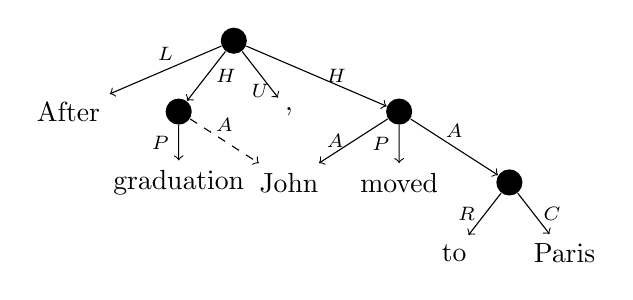
\begin{tikzpicture}[level distance=9mm, sibling distance=14mm, ->,
        every circle node/.append style={fill=black}]
      \tikzstyle{word} = [font=\rmfamily,color=black]
      \node (ROOT) [circle] {}
        child {node (After) [word] {After} edge from parent node[above] {\scriptsize $L$}}
        child {node (graduation) [circle] {}
        {
          child {node [word] {graduation} edge from parent node[left] {\scriptsize $P$}}
        } edge from parent node[right] {\scriptsize $H$} }
        child {node [word] {,} edge from parent node[below] {\scriptsize $U$}}
        child {node (moved) [circle] {}
        {
          child {node (John) [word] {John} edge from parent node[left] {\scriptsize $A$}}
          child {node [word] {moved} edge from parent node[left] {\scriptsize $P$}}
          child {node [circle] {}
          {
            child {node [word] {to} edge from parent node[left] {\scriptsize $R$}}
            child {node [word] {Paris} edge from parent node[right] {\scriptsize $C$}}
          } edge from parent node[above] {\scriptsize $A$} }
        } edge from parent node[right] {\scriptsize $H$} }
        ;
      \draw[dashed,->] (graduation) to node [above] {\scriptsize $A$} (John);
    \end{tikzpicture}
\caption{\label{fig:example_ucca}
 Example UCCA graph. The dashed edge is remote.
%  Pre-terminal nodes and edges are omitted for brevity.
  }
\end{figure}

%%%%%%%%%%%%%%%%%%%%%%%%%%%%%%%%%%%%%%%%%%%%%%%%%%%%%%%%%%%%%%%%
\paragraph{Universal Dependencies.}\label{sec:ud}
UD \cite{nivre2016universal} has quickly become
the dominant dependency scheme for
syntactic  annotation in many languages,
aiming for cross-linguistically consistent and coarse-grained treebank
annotation. Formally, UD uses bilexical trees, with edge labels 
representing syntactic relations between words.
Figure~\ref{fig:original_example_ud} shows an example UD tree.


\begin{figure}[!ht]

\fbox{\begin{subfigure}{0.47\textwidth}
  \centering
    \begin{dependency}[text only label, label style={above}, font=\small]
    \begin{deptext}[column sep=.8em,ampersand replacement=\^]
    After \^ graduation \^ , \^ John \^ moved \^ to \^ Paris \\
    \end{deptext}
        \depedge[edge unit distance=1ex]{2}{1}{case}
        \depedge[edge unit distance=1ex]{4}{3}{punct}
        \depedge[edge unit distance=1ex]{5}{4}{nsubj}
        \depedge[edge unit distance=1ex, edge end x offset=-2pt]{2}{5}{obl}
        \depedge[edge unit distance=1ex]{7}{6}{case}
        \deproot[edge unit distance=1.5ex]{5}{root}
        \depedge[edge unit distance=1.5ex]{5}{7}{obl}
    \end{dependency}
  \caption{UD \label{fig:original_example_ud}}
\end{subfigure}}

\fbox{\begin{subfigure}{0.47\textwidth}
  \centering
  \scalebox{.95}{
  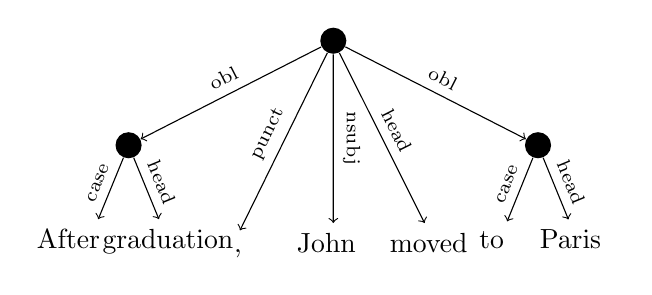
\begin{tikzpicture}[level distance=15mm, ->,
      every node/.append style={sloped,anchor=south,auto=false,font=\scriptsize},
      level 1/.style={sibling distance=13mm},
      level 2/.style={sibling distance=1cm}]
    \tikzstyle{word} = [font=\rmfamily,color=black]
    \node (ROOT) [fill=black,circle] {}
      child {node (after) [fill=black,circle] {}
      {
        child {node [word] {After{\color{white}g}\quad\quad} edge from parent node {case}}
        child {node [word] {\quad graduation\quad\quad} edge from parent node {head}}
      } edge from parent node {obl}}
      child {node {}
      {
        child {node [word] (comma) {\quad,{\color{white}g}} edge from parent [draw=none]}
      } edge from parent [draw=none]}
      child {node {}
      {
        child {node [word] (John) {John{\color{white}g}} edge from parent [draw=none]}
      } edge from parent [draw=none]}
      child {node {}
      {
        child {node [word] (moved) {moved{\color{white}g}} edge from parent [draw=none]}
      } edge from parent [draw=none]}
      child {node (to) [fill=black,circle] {}
      {
          child {node [word] {to{\color{white}g}} edge from parent node {case}}
          child {node [word] {Paris{\color{white}g}} edge from parent node {head}}
      } edge from parent node {obl}}
      ;
      \draw (ROOT) to node {punct} (comma);
      \draw (ROOT) to node {nsubj} (John);
      \draw (ROOT) to node {head} (moved);
  \end{tikzpicture}}
  \captionof{figure}{UD}\label{fig:converted_example_ud}
\end{subfigure}}

\caption{Figure \ref{fig:original_example_ud} presents a UD tree.
  Edge labels express syntactic relations.
Figure~\ref{fig:converted_example_ud} presents a converted UD graph.
%(with pre-terminals omitted: each terminal drawn in place of its parent).
Intermediate non-terminals and \textit{head} edges are introduced.
%While converted UD graphs form trees, enhanced++ UD graphs may not.
}\label{fig:ud_examples}
\end{figure}


%%%%%%%%%%%%%%%%%%%%%%%%%%%%%%%%%%%%%%%%%%%%%%%%%%%%%%%%%%%%%%%%%%%%%%%%%%%%%%%%%%%%%%%%%%%%%%5
\section{Shared Gold Standard Corpus}\label{sec:shared}

We annotate 804 English sentences from the \textit{reviews} section of the 
English Web Treebank \cite[EWT; ][]{bies2012english}.
The sentences are annotated by two UCCA annotators and
cross-reviewed.\footnote{The data will be released upon publication.}
As these sentences are included in the Universal Dependencies 
English\_EWT treebank, we have both gold-standard UCCA and UD for them. 
We refer to this set as \textit{shared} henceforth.
The data contains 11,103 tokens, constituting 4\% of the full UD English\_EWT treebank,
and 20\% of its \textit{reviews} section
(see Table~\ref{tab:corpora}).


%%%%%%%%%%%%%%%%%%%%%%%%%%%%%%%%%%%%%%%%%%%%%%%%%%%%%%%%%%%%%%%%%%%%%%%%%%%%%%%%%%%%%%%%%%%%%%5
\section{Comparison Methodology}\label{sec:methodology}

To facilitate comparison between UCCA and UD,
we first assimilate the graphs by abstracting away from formalism differences,
obtaining a similar graph format for both schemes,
over the tokens of the sentence.
We then match pairs of nodes in the converted UD and UCCA trees
if they share the same set of terminals in their yields (\S\ref{sec:analysis}).

One obvious difference is that UD annotates bi-lexical dependency graphs,
while UCCA graphs contain non-terminal nodes.
To reach a common format, we use the unified DAG format by
\citet{hershcovich2018multitask},\footnote{\url{http://github.com/huji-nlp/semstr}}
outlined in \S\ref{sec:conversion}.
Then, in \S\ref{sec:local}, we describe our extended converter,
developed following inspection of the formal differences between
UCCA and the basic converted UD trees,
to remove non-content differences.

\subsection{Remotes and Enhanced Dependencies}\label{sec:remote}

In the UCCA format, edges are labeled (but not nodes),
and are divided into \textit{primary} and \textit{remote} edges
(e.g., the dashed edge in Figure~\ref{fig:example_ucca}),
where the primary edges form a tree (all nodes have at most one primary parent,
and the root has none).
Remote edges enable reentrancy, and thus together with primary edges form a DAG.

UD includes
\textit{enhanced dependencies}\footnote{\url{http://universaldependencies.org/u/overview/enhanced-syntax.html}}
\cite{SCHUSTER16.779}
%as part of the dependency graph,
representing case information, elided predicates,
and shared arguments due to conjunction, control, raising and relative clauses.
%They provide richer information to downstream semantic applications,
%making UD better suited for text understanding.
Enhanced UD has a more restricted notion of shared arguments than UCCA's.

In order to facilitate comparison,
%and as UD does not support reentrancy,\footnote{Reentracy is supported by enhanced UD .}
we remove remote edges and enhanced dependencies in the conversion process.
Future work will explore the differences and commonalities between them.


%\oa{move this paragraph some place else}
%  UCCA graphs are converted into trees by removing ``remote edges''.
%  Remote edges in UCCA encode shared argumenthood by assigning multiple parents to the same node. Such phenomena are largely ignored in UD, %which uses trees. See \S\ref{sec:analysis}.


\subsection{Basic Conversion}\label{sec:conversion}

Figure~\ref{fig:converted_example_ud} presents an example UD tree conversion.
Given a UD tree, the converter adds a pre-terminal for each token,
and attaches the pre-terminals according to the original dependency edges:
traversing the tree from the root down, for each head token it creates a non-terminal
parent with the edge label {\it head}, and adds the node's dependents as children of 
the created non-terminal node.
%Any \textit{enhanced}
%heads beyond the normal head of a node are converted to remote edges in the unified DAG format.
In the conversion process, any language-specific relation subtypes are stripped,
leaving only the universal relations.
For example, the language-specific label for definite artciles
\texttt{det:def} is replaced by the universal relation \texttt{det}.

%%%%%%%%%%%%%%%%%%%%%%%%%%%%%%%%%%%%%%%%%%%%%%%%%%%%%%%%%%%%%%%%%%%%%%%%%%%%%%%
\subsection{Local Modifications}\label{sec:local}

We extend the converter to remove further formalism differences.

\paragraph{Unanalyzable units.}
Unanalyzable phrases are represented in UCCA as a single unit covering multiple terminals.
In UD, each word after the first is attached to the previous word,
with the \texttt{flat}, \texttt{fixed} or \texttt{goeswith} relations
(depending on whether the phrase is a name or a title, or whether it is one word split by error).
During conversion, we remove edges of both relations and group the corresponding terminals to one unit.
Multi-word expressions also include compounds, discussed in \S\ref{sec:mwe}.

\paragraph{Promotion of function words.}
In general, the basic conversion protocol attaches low,
selecting for each terminal $t$ the lowest non-terminal of which $t$
is the head terminal.
To abstract away from convention differences,
we extend the conversion protocol by adding special rules
promoting the dependents of \texttt{cc} relations,
and of \texttt{mark} dependents with an \texttt{advcl} head
(e.g. ``when'', ``if'', ``after'', and purposive ``to''),
as there is a systematic mapping between the UCCA and UD guidelines
and it is different from the default low-attaching behavior.
%Selecting a forward-attaching behavior instead:
%\begin{itemize}
%  \item Conjunctions (\texttt{cc} in UD) attach to the following
%  conjuncts (word with an incoming \texttt{conj} relation).
%  \item \texttt{mark} is attached to the following \texttt{advcl}.
%\end{itemize}
%These rules are applied to the bilexical graph after the conversion process.


\section{Analysis of Divergences}\label{sec:analysis}

In this section, we analyze in detail the content differences between UCCA and UD,
as quantified in a \textit{confusion matrix} between the schemes (\S\ref{sec:confusion}).

The analysis excludes the following relations,
as they are irrelevant to the evaluation of content differences:

\begin{description}
  \item[root.] Always matches the whole sentence.
  \item[punct.] No semantic content; excluded from UCCA evaluation.
  \item[fixed, flat and goeswith.] Correspond to parts of unanalyzable units in UCCA,
  and so not represented as units on their own.
  The UD distinction is between, respectively, fixed grammatical expressions,
  semi-fixed MWEs like names, titles or dates, and erroneously separated words (see \S\ref{sec:local}).
  \item[dep and orphan.] Rare; no consistent relation.
\end{description}

\begin{table}[t]
\centering
\scriptsize
\setlength\tabcolsep{2pt}
\begin{tabular}{l|ccccccccccccc}
 & \rotatebox{90}{Participant (A)} & \rotatebox{90}{Center (C)}
 & \rotatebox{90}{Adverbial (D)} & \rotatebox{90}{Elaborator (E)}
 & \rotatebox{90}{Function (F)} & \rotatebox{90}{Ground (G)}
 & \rotatebox{90}{Linked Scene (H)} & \rotatebox{90}{Linker (L)}
 & \rotatebox{90}{Connector (N)} & \rotatebox{90}{Process (P)}
 & \rotatebox{90}{Relator (R)} & \rotatebox{90}{State (S)} & \rotatebox{90}{{\sc NoMatch}} \\
\hline
acl & 8 & 0 & 0 & 101 & 2 & 0 & 15 & 0 & 0 & 0 & 0 & 1 & 49 \\
advcl & 2 & 2 & 0 & 0 & 0 & 0 & 103 & 1 & 0 & 4 & 0 & 0 & 97 \\
advmod & 61 & 9 & 524 & 53 & 12 & 33 & 3 & 61 & 0 & 2 & 6 & 5 & 71 \\
amod & 1 & 33 & 106 & 218 & 2 & 0 & 7 & 0 & 0 & 3 & 0 & 97 & 61 \\
appos & 1 & 10 & 1 & 8 & 0 & 0 & 5 & 0 & 0 & 0 & 0 & 4 & 10 \\
aux & 0 & 0 & 96 & 0 & 285 & 0 & 0 & 0 & 0 & 0 & 0 & 0 & 2 \\
case & 1 & 5 & 2 & 15 & 34 & 0 & 0 & 48 & 6 & 1 & 489 & 50 & 75 \\
cc & 0 & 0 & 1 & 1 & 0 & 0 & 0 & 305 & 71 & 0 & 1 & 0 & 11 \\
ccomp & 78 & 0 & 0 & 0 & 0 & 0 & 8 & 0 & 0 & 0 & 0 & 1 & 41 \\
compound & 23 & 24 & 11 & 174 & 2 & 0 & 0 & 0 & 0 & 1 & 1 & 3 & 167 \\
conj & 2 & 88 & 1 & 0 & 0 & 0 & 265 & 0 & 0 & 2 & 0 & 3 & 90 \\
cop & 0 & 0 & 0 & 0 & 333 & 0 & 0 & 0 & 0 & 3 & 1 & 24 & 3 \\
csubj & 2 & 0 & 0 & 0 & 0 & 0 & 0 & 0 & 0 & 0 & 0 & 0 & 8 \\
det & 2 & 1 & 23 & 778 & 1 & 1 & 0 & 0 & 0 & 0 & 2 & 0 & 26 \\
discourse & 0 & 1 & 0 & 0 & 1 & 6 & 13 & 3 & 0 & 0 & 0 & 1 & 1 \\
expl & 0 & 0 & 0 & 0 & 22 & 0 & 0 & 0 & 0 & 0 & 0 & 0 & 2 \\
iobj & 19 & 0 & 0 & 0 & 0 & 0 & 0 & 0 & 0 & 0 & 0 & 0 & 0 \\
list & 0 & 2 & 0 & 0 & 0 & 0 & 8 & 0 & 0 & 0 & 0 & 0 & 2 \\
mark & 0 & 2 & 4 & 0 & 161 & 1 & 0 & 159 & 1 & 0 & 53 & 1 & 18 \\
nmod & 100 & 1 & 5 & 231 & 0 & 0 & 6 & 0 & 0 & 0 & 0 & 3 & 112 \\
nsubj & 993 & 0 & 0 & 0 & 14 & 0 & 2 & 9 & 0 & 3 & 24 & 1 & 37 \\
nummod & 4 & 7 & 3 & 53 & 0 & 0 & 3 & 0 & 0 & 0 & 0 & 0 & 24 \\
obj & 439 & 7 & 10 & 1 & 1 & 0 & 1 & 1 & 0 & 8 & 6 & 0 & 92 \\
obl & 247 & 1 & 92 & 8 & 2 & 4 & 4 & 4 & 0 & 0 & 2 & 0 & 132 \\
parataxis & 1 & 0 & 0 & 1 & 0 & 2 & 79 & 0 & 0 & 1 & 0 & 2 & 39 \\
vocative & 9 & 0 & 0 & 0 & 0 & 3 & 0 & 0 & 0 & 0 & 0 & 0 & 0 \\
xcomp & 44 & 1 & 2 & 2 & 0 & 0 & 1 & 0 & 0 & 5 & 0 & 7 & 116 \\
head & 125 & 1,401 & 157 & 51 & 91 & 18 & 459 & 2 & 1 & 961 & 9 & 354 & 729 \\
{\sc NoMatch} & 329 & 173 & 53 & 73 & 6 & 5 & 673 & 29 & 0 & 141 & 7 & 98
\end{tabular}
\caption{UD-UCCA confusion matrix calculated from EWT
gold-standard annotations (\S\ref{sec:shared}),
after converting UD to the unified DAG format,
by comparing incoming edge labels for units with the same terminal yields.
The last column (row) show the number of edges of each UD (UCCA) category
that do not match any UCCA (UD) unit.
\label{tab:confusion_matrix}}
\end{table}

\subsection{Confusion Matrix}\label{sec:confusion}

Using the standard UCCA evaluation
script,\footnote{\url{http://github.com/huji-nlp/ucca/blob/master/scripts/evaluate_standard.py}}
we create a confusion matrix between the edge tags in converted UD graphs
and the annotated UCCA graphs (see Table~\ref{tab:confusion_matrix}).
We perform this analysis on gold UD and UCCA graphs from the shared EWT corpus
(see \S\ref{sec:shared}),
after conversion to the unified DAG format.
Excluding punctuation, this gives 13293 yields in UCCA and
9817 in UD.
Of these, 8416 are common, meaning that an oracle would get an $F_1$ score
of 72.8\% if it had the gold label for each edge on conversion.

In the following subsections, we categorize the UD relations according to their
treatment in UCCA, examining the main distinctions different between the schemes.

\subsection{Scenes/non-Scenes}\label{sec:scenes}

UCCA distinguishes between Scenes (descriptions of events, states or activities)
and non-Scenes. 
This distinction cuts across UD categories,
as a Scene can be evoked by a verb, an eventive or stative
noun (``negotiation'', ``fatigue''),
an adjective or even a preposition (``this is \textit{for} John'').
\begin{description}
    \item[iobj, nsubj, and obj.]
    Core syntactic arguments are usually semantic arguments,
    i.e., Participants (e.g., ``\textit{Wine} was excellent'').
    However, when describing a scene, such a phrase is a Process/State
    (e.g., ``But \textit{service} is very poor'').
    Some wh-pronouns are the subject or object of a relative clause, and
    are analyzed as Linkers or Relators,
    depending on whether they modify a scene or non-scene, respectively
    (e.g., ``Overall, Joe is a happy camper \textit{who} has found a great spot''
    and ``one of the staff \textit{who} was very pleasant and professional'').
    \item[amod.]
    Adjectival modifiers of nominals are Adverbials or Elaborators,
    depending on whether they modify scenes or non-scenes, respectively
    (``\textit{romantic} dinner'' vs. ``\textit{medical} school''), or
    as States when
    they evoke scenes on their own (``\textit{beautiful} hotel'').
    \item[nmod and acl.]
    Nominal and clausal modifiers of nominals
    are generally split between Participants and Elaborators,
    depending on whether they modify scenes
    (e.g., ``discount \textit{on services}'' and
    ``our decision \textit{to buy when we did}'')
    or non-scenes (e.g., ``\textit{my car's} gears and brakes'' and
    ``Some of the younger kids \textit{that work there}'').
    Many unmatched adjectival clauses are
    \textit{fused relative clauses},
    (e.g., ``The prices were worth what \textit{I got}'',
    where \textit{what} is the object of \textit{worth} in UD but
    is a Participant of \textit{I got} in UCCA).
    \item[case.]
    While most case markers are Relators,
    modifying non-scene units (e.g., ``the team \textit{at} Bradley Chevron''),
    some are Linkers as they modify a scene
    (e.g., ``Very informative website \textit{with} a lot of good work'').
    Some are semantically vacuous and annotated as Functions
    (e.g., ``a large group \textit{of} my friends''),
    while others are Elaborators (e.g., ``\textit{over} a year''),
    or Processes/States
    (e.g., ``not at all \textit{like} the junk you get at the grocery stores'').
    \item[cc, conj and list.]
    Coordinating conjunctions are either Connectors, between non-scenes
    (e.g., ``Mercedes \textit{and} Dan'')
    or Linkers, between scenes
    (e.g., ``outdated \textit{but} not bad'').
    Correspondingly, conjuncts (and list elements)
    are Centers or Linked Scenes (H).\footnote{Note
    that while in UD the dependent \texttt{cc} is attached to the following conjunct,
    in UCCA coordination is a flat structure.
    This is a convention difference that we fixed with local modifications
    (\S\ref{sec:local})---otherwise most \texttt{conj} instances would be unmatched,
    containing the coordinating conjunction which is outside the unit in UCCA.}
    \item[det.]
    While usually Elaborators,
    determiners are Adverbials when modifying a scene
    (e.g., ``\textit{no} feathers in stock'').
\end{description}

\subsection{Arguments/Adjuncts}\label{sec:arguments}

While UD distinguishes core arguments and non-core dependents of clausal predicates,
UCCA distinguishes Participants,
including locations and abstract entities,
from secondary relations (Adverbials), 
which cover manner, aspect and modality.
Secondary relations can be verbs (e.g., ``begin'', ``fail''),
prepositional phrases (``with disrespect''),
as well as modals, adjectives and adverbs.
\begin{description}
    \item[aux.]
    Auxiliary verbs are Functions (e.g., ``\textit{do} not forget''),
    or Adverbials when they semantically modify a scene
    (e.g., ``you \textit{can} graduate'').
    \item[advmod and obl.]
    While in the majority of cases,
    adverbial modifiers correspond to semantic Adverbials
    (e.g., ``I \textit{sometimes} go''),
    they may be Participants,
    mostly in the case of semantic arguments describing location.
    Oblique nominals, on the other hand, mostly correspond to Participants
    (e.g., ``wait \textit{for Nick}), but may be
    Adverbials, mostly in case of adjuncts describing time.
    In ``went \textit{there yesterday}'',
    the adverbial modifier ``\textit{there}'' is a Participant,
    while the oblique ``\textit{yesterday}'' as an Adverbial.
    \item[csubj, ccomp and xcomp.]
    As they are core arguments of predicates,
    in most cases, (open) clausal subjects and complements are Participant scenes
    (e.g., ``it was great \textit{that they did not charge a service fee}'',
    ``did not really know \textit{what I wanted}'' or
    ``I asked them \textit{to change it}'').
    However, when modifying a secondary verb (which would be an Adverbial),
    they may not correspond to a whole unit, or if the clause is a single word,
    correspond to Process/State
    (e.g., ``She makes \textit{every item fit you perfectly}'' or
    ``this seems \textit{great}'').
    \item[vocative.]
    Vocatives are annotated as Ground,
    but also as Participants if they are arguments in a scene
    (e.g., ``Thanks \textit{Mark}'').
\end{description}    
    

\subsection{Multi-Word Expressions}\label{sec:mwe}

UD and UCCA treat multi-word expressions (MWEs) differently.
MWEs in UD include names, compounds and grammaticalized fixed expressions.
UCCA treats names and grammaticalized MWEs as unanalyzable units,
but also a range of semantically opaque constructions
(e.g., light verbs and idioms).
On the other hand, compounds are not necessarily unanalyzable in UCCA,
especially where they are compositional.
\begin{description}
    \item[compound.]
    This is a very heterogenous category.
    Most compounds correspond to Elaborators (e.g., ``\textit{industry} standard''),
    and many are unanalyzable expressions (e.g., ``figure \textit{out}'').
    In many cases, a compound represent an argument,
    and is annotated as a Participant (e.g., ``\textit{food} craving'')
    or it may be a State (e.g., ``\textit{out-of-place} flat-screen TV''),
    while in other cases it is an Adverbial (e.g., ``\textit{first time} buyers'').
    In nested compounds, a dependent may be itself a co-Center
    within an Elaborator
    (e.g., ``\textit{sweet potato} tempura roll'').
    \item[case, det, nsubj, and obj.]
    Many of these are unanalyzable due to UCCA's stronger tendency to group
    multi-word expressions (e.g., ``lots \textit{of}'',
    ``\textit{a} bit'', ``when \textit{it} comes to'', ``bites \textit{the dust}'',
    respectively).
    \item[nummod.]
    Numeric modifiers are mostly Elaborators, but often do not correspond to a whole UCCA unit
    due to Adverbials in a flat structure (e.g., ``about \textit{50}\%'').
\end{description}

\subsection{Linkage}\label{sec:linkage}

UD categorizes clause linkage into coordination,
subordination, argumenthood (complementation),
and parataxis (a residual category).
UCCA only distinguishes between argumenthood 
and largely conflates clausal coordination, subordination and parataxis.
\begin{description}
    \item[mark.]
    UCCA distinguishes between the infinitive marker ``to'', annotated as Function,
    and the use of markers for inter-scene linkage, such as purposive ``to'',
    annotated as Linker
    (e.g., in ``how much they want me \textit{to} pay \textit{to} fix this thing'',
    the first \textit{to} is a Function and the second is a Linker).\daniel{still
    struggling to find an R mark that shouldn't actually be an L}
    \item[advcl and parataxis.]
    Both adverbial clauses and parataxis almost exclusively Linked Scene
    (e.g., ``We called few companies before \textit{we decided to hire them}''
    and ``Check out The Willow Lounge, \textit{you'll be happy}'')\footnote{Note
    that while in UD the dependent \texttt{mark}, e.g. ``before'',
    is attached to the following adverbial clause,
    in UCCA linkage is a flat structure.
    This is a convention difference that we fixed with local modifications
    (\S\ref{sec:local})---otherwise most \texttt{advcl} instances would be unmatched,
    containing the linker which is outside the scene in UCCA.}.
\end{description}
    

\subsection{Other Distinctions}\label{sec:misc}

\begin{description}
    \item[appos.]
    Appositional modifiers are always analyzed in UD such that
    the modifier nominal follows the modified noun.
    In UCCA, these are split between Center
    (``its sister store \textit{Peking Garden}'')
    and Elaborator (``Kevin, \textit{the manager}''),
    as a named entity will be the Center regardless of the order.
    \item[cop.]
    UCCA distinguishes between copular constructions expressing
    identity (e.g., ``It \textit{was} an ingrown toenail'') where the copula is annotated as State
    (and the head is a Participant),
    as opposed to attributes or set membership
    (e.g., ``Mercedes and Dan \textit{are} very thorough''), where it is annotated as Function
    (and the head is a State).    
    \item[discourse.]
    Interjections and discourse markers are given the categories of
    Linked Scene, Ground or Linker,
    if they are, respectively, a complete scene or part of a scene relating to the \textit{speech event}
    (e.g., ``\textit{no}, Warwick in New Jersey'' and
    ``\textit{Please} visit my website''),
    or simply relate one scene to another
    (e.g., ``I am sure, \textit{well}, she says'').
    \item[expl and nsubj.]
    Expletives are Functions in UCCA, lacking semantic content.
    Some instances of ``it'' and ``that'', analyzed as subjects in UD,
    are analyzed as expletives in UCCA, and annotated as Function
    (e.g., ``\textit{it}'s like driving a new car'').    
    \item[head.]
    While not a UD relation, this label is introduced on the conversion from dependency graphs
    \cite{hershcovich2018multitask}.
    For any word with at least one dependent,
    a non-terminal node will be created in the converted graph, with a \textit{head} edge.
    About 17\% of these edges are unmatched, mostly due to unanalyzable expressions and inter-scene linkage.
    About 70\% are Process, State, Linked Scene or Center,
    where the notion of syntactic head matches that of a ``UCCA head''.
    In the remaining case there is a content difference between the schemes
    (e.g., ``\textit{all} of Dallas'', where \textit{all} is an Elaborator
    in UCCA but is the syntactic head in UD).
\end{description}


%\section{Full Conversion}\label{sec:conversion}
%
%The conversion protocol introduced in \S\ref{sec:methodology} outputs graphs in a UCCA-like
%format, but with UD edge labels.
%In this section we describe a full conversion protocol,
%aiming at reaching ``native'' UCCA graphs.
%
%\paragraph{Label mapping.}
%The confusion matrix introduced in \S\ref{sec:confusion}
%provides a distribution of the possible UCCA categories
%corresponding to each UD relation.
%By finding the mode of this distribution,
%we get the most likely translation.
%To convert the UD trees into fully labeled UCCA graphs,
%we replace each UD relation with its most common UCCA counterpart.
%
%\paragraph{Postprocessing.}
%The \textit{head} edges introduced as part of the conversion (\S\ref{sec:conversion})
%do not have a single
%corresponding UCCA edge label---although Center is the most common corresponding label,
%other labels such as Process are also common.
%This is a difference between UD, which selects the most central token to be the head of a phrase,
%to UCCA, which also annotates the relation between that head and the unit it is part of.
%To overcome this limitation, we replace all \textit{head} labels with C, but then
%apply standard UCCA
%normalization\footnote{\url{https://github.com/huji-nlp/ucca/blob/master/scripts/normalize.py}}
%to the resulting graphs after conversion,
%replacing Center with Process when it has sibling Participants or
%with Linked Scene when it has sibling Linked Scenes.
%We select Process rather than State as the main relation in the normalization because
%it is much more common (14,719 Processess in the Wiki corpus as opposed to 3354 States).




%\section{Improving UCCA Parsing with UD}\label{sec:silver}

%Syntactic dependency parsers require many training examples to achieve
%state-of-the-art results.
%Even after around 500K tokens, the learning curves do not seem to saturate
%\cite{de2017old,velldal2017joint}.
%
%Whereas the largest UCCA training set (English Wiki) contains 128K tokens,
%The largest joined English UD training set (EWT) contains 177K tokens.
%In French UCCA has just 10K training tokens whereas UD has 295K,
%and in German UCCA has 80K and UD 228K.
%
%\begin{table}[t]
%\centering
%\begin{tabular}{l|lll|lll}
%& \multicolumn{3}{c|}{\footnotesize \bf Primary} & \multicolumn{3}{c}{\footnotesize \bf Remote} \\
%& \footnotesize \textbf{LP} & \footnotesize \textbf{LR} & \footnotesize \textbf{LF}
%& \footnotesize \textbf{LP} & \footnotesize \textbf{LR} & \footnotesize \textbf{LF} \\
%\hline
%\footnotesize 10\% & 65.1 & 65.2 & 65.1 & 38.4 & 24.3 & 29.8\\
%\footnotesize 20\% & 68.9 & 68.3 & 68.6 & 47.1 & 28.0 & 35.2\\
%\footnotesize 30\% & 70.2 & 70.1 & 70.2 & 47.2 & 45.5 & 46.3\\
%\footnotesize 40\% & 71.5 & 71.3 & 71.4 & 52.5 & 46.1 & 49.1\\
%\footnotesize 50\% & 71.9 & 71.9 & 71.9 & 51.3 & 48.6 & 49.9\\
%\footnotesize 60\% & 71.3 & 72.4 & 71.9 & 52.9 & 45.5 & 48.9\\
%\footnotesize 70\% & 73.1 & 72.7 & 72.9 & 50.8 & 50.5 & 50.6\\
%\footnotesize 80\% & 73.5 & 72.6 & 73.0 & 52.8 & 47.0 & 49.8\\
%\footnotesize 90\% & 73.9 & 73.1 & 73.5 & 52.3 & 48.6 & 50.4\\
%\footnotesize 100\% & 74.7 & 74.8 & 74.8 & 48.5 & 51.2 & 49.8\\
%\end{tabular}
%\caption{
%Development scores for TUPA \protect\cite{hershcovich2017a} when trained on increasing amount of training data
%(English Wiki corpus).
%\label{tab:partial_data_results}}
%\end{table}
%
%Table~\ref{tab:partial_data_results} shows results for TUPA,
%trained on 10\%, 20\% etc. of the Wiki training set and tested on the Wiki development set.
%As can be seen, the primary labeled F1 continues improving substantially even from 90\% to 100\%
%of the training data. More training data is likely to yield even better performance.

%%%%%%%%%%%%%%%%%%%%%%%%%%%%%%%%%%%%%%%%%%%%%%%%%%%%%%%%%%%%%%%%%%%%%%%%%%%%%%%%%
\section{Fine-Grained UCCA Evaluation}\label{sec:fine_grained}

\subsection{Experimental Setup}\label{sec:experiments}

\begin{table*}[t]
\centering
\small
\setlength\tabcolsep{2pt}
\begin{tabular}{l|ccc|ccc||ccc|ccc||ccc|ccc}
& \multicolumn{6}{c||}{\footnotesize \bf English}
& \multicolumn{6}{c||}{\footnotesize \bf French}
& \multicolumn{6}{c}{\footnotesize \bf German} \\
\hline
& \multicolumn{3}{c|}{\footnotesize \bf {\#} tokens}
& \multicolumn{3}{c||}{\footnotesize \bf {\#} sentences}
& \multicolumn{3}{c|}{\footnotesize \bf {\#} tokens}
& \multicolumn{3}{c||}{\footnotesize \bf {\#} sentences}
& \multicolumn{3}{c|}{\footnotesize \bf {\#} tokens}
& \multicolumn{3}{c}{\footnotesize \bf {\#} sentences} \\
& \footnotesize \bf train & \footnotesize \bf dev & \footnotesize \bf test
& \footnotesize \bf train & \footnotesize \bf dev & \footnotesize \bf test
& \footnotesize \bf train & \footnotesize \bf dev & \footnotesize \bf test 
& \footnotesize \bf train & \footnotesize \bf dev & \footnotesize \bf test
& \footnotesize \bf train & \footnotesize \bf dev & \footnotesize \bf test
& \footnotesize \bf train & \footnotesize \bf dev & \footnotesize \bf test \\
\hline
%UCCA &&&&&&&&&&&&&&&&&& \\
Wiki & 124935 & 17784 & 15854 & 4113 & 514 & 515 &&&&&&&&&&&& \\
%Wiki 1.2.0 & 128444 & 14676 & 15313 & 4268 & 454 & 503 &&&&&&&&&&&& \\
20K && 12574 &&& 492 & 618 & 6374 & 5962 & 15 & 238 & 239 & 119872 & 12334 & 12325 & 5211 & 651 & 652 \\
%\multicolumn{2}{l}{20K 1.0.0/0.9.0} && 12339 &&& 506 & 10047 & 1558 & 1324 & 413 & 67 & 67 & 79894 & 10059 & 42366 & 3429 & 561 & 2164 \\
%\hline
%UD 2.3 & \multicolumn{2}{l}{152141} && \multicolumn{2}{l}{12543} &&
%\multicolumn{2}{l}{250658} && \multicolumn{2}{l}{14450} && \multicolumn{2}{l}{209131} && 13814 \\
%\hline
EWT &&& 11103 &&& 804 &&&&&&&&&&&&
\end{tabular}
\caption{Number of tokens and sentences in the training, development and test sets
we use for each corpus and language.\label{tab:corpora}}
\end{table*}

\paragraph{Data.}

We use v1.2.3 of the UCCA English Wikipedia corpus (\textit{Wiki}),
with the standard train/dev/test split (see Table~\ref{tab:corpora}),
and the \textit{Twenty Thousand Leagues Under the Sea} corpora (\textit{20K}),
annotated in English (v1.2.2), French (v1.2.2)
and German (v1.0.1).\footnote{\url{http://github.com/UniversalConceptualCognitiveAnnotation}}

%For comparability with previous work \cite{hershcovich2017a,hershcovich2018multitask},
%we also perform our experiments on Wiki v1.2.0 \cite{abend2013universal},
%on 20K v1.0.0 in English and French \cite{sulem2015conceptual},
%and on 20K v0.9.0 in German.
%As in previous work, we use English 20K only as an out-of-domain test set.

%For UD, we use the English\_EWT, French\_GSD and German\_GSD
%treebanks from Universal Dependencies v2.3
%\cite{11234/1-2895}.\footnote{\url{http://hdl.handle.net/11234/1-2895}}
%These are the largest freely-available UD treebanks for these languages.


%\paragraph{Evaluation of gold UD annotations.}
%
%We apply our conversion protocol (\S\ref{sec:methodology}) to
%the gold-standard UD trees of the English EWT shared sentences,
%and evaluate on the gold-standard UCCA for the same sentences.
%We then apply the label mapping to get fully labeled converted UCCA graphs.

\paragraph{Evaluation by automatically parsed UD.}

To perform fine-grained analysis on the UCCA corpora that do not have gold-standard UD,
we use UDPipe v1.2 \cite{udpipe,udpipe:2017}, trained on the UD v2.3 treebanks.

%\paragraph{Baselines.}
%
%As a point of comparison, we evaluate TUPA \cite{hershcovich2017a} on the test sets,
%after training it on the UCCA training set for each language (Wiki for English,
%and 20K for French and German).
%For equal conditions,
%we train and test TUPA using features predicted by UDPipe,
%yielding slightly lower scores than previously reported using spaCy.%\footnote{\url{https://spacy.io}}

%\paragraph{Using converted UD as ``silver-standard'' data.}
%
%Using our conversion protocol (\S\ref{sec:conversion}),
%we convert the gold-standard UD graphs into UCCA.
%We use the converted UD data as ``silver-standard'' data \cite{W17-7306,N18-1104}
%and add it to the UCCA training set for training TUPA.

\subsection{Results}\label{sec:results}


\begin{table}[t]
\centering
\begin{tabular}{l|lll|lll}
& \multicolumn{3}{c|}{\footnotesize \bf Primary} & \multicolumn{3}{c}{\footnotesize \bf Remote} \\
& \footnotesize \textbf{UP} & \footnotesize \textbf{UR} & \footnotesize \textbf{UF}
& \footnotesize \textbf{UP} & \footnotesize \textbf{UR} & \footnotesize \textbf{UF} \\
\hline
\multicolumn{4}{l|}{\small \bf English EWT (shared)} & \\
\footnotesize UD 2.3
& 81.5 & 88.2 & 84.7 & 21.2 & 19.6 & 20.4 \\
\footnotesize TUPA
& 83.4 & 82.6 & 83 & 46.4 & 18.6 & 26.6 \\
\multicolumn{4}{l|}{\small \bf English Wiki test} & \\
\footnotesize UDPipe
& 76.5 & 81.2 & 78.8 & -- & -- & -- \\
\footnotesize TUPA
& 87.1 & 84.5 & 85.8 & 50.9 & 46.2 & 48.4 \\
\multicolumn{4}{l|}{\small \bf English 20K} & \\
\footnotesize UDPipe
& 79.2 & 85.1 & 82.1 & -- & -- & -- \\
\footnotesize TUPA
& 83.2 & 83.8 & 83.5 & 46.6 & 16.5 & 24.3 \\
\multicolumn{4}{l|}{\small \bf French 20K test} & \\
\footnotesize UDPipe
& 78.8 & 84.3 & 81.5 & -- & -- & -- \\
\footnotesize TUPA
& 72.8 & 65.4 & 68.9 & 23.5 & 3.5 & 6 \\
\multicolumn{4}{l|}{\small \bf German 20K test} & \\
\footnotesize UDPipe
& 80.5 & 85.2 & 82.8 & -- & -- & -- \\
\footnotesize TUPA
& 88.2 & 85.3 & 86.7 & 68.3 & 37.2 & 48.2
\end{tabular}
\caption{
Unlabeled precision, recall and $F_1$ (in~\%) for primary and remote edges.
UD 2.3 is the gold-standard UD (v2.3) after conversion to UCCA by our protocol.
For comparison, TUPA \protect\cite{hershcovich2017a} is trained on Wiki with features predicted by UDPipe
and tested with predicted POS and dependency features.
\label{tab:conversion_results_unlabeled}}
\end{table}

%\begin{table}[t]
%\centering
%\begin{tabular}{l|lll|lll}
%& \multicolumn{3}{c|}{\footnotesize \bf Primary} & \multicolumn{3}{c}{\footnotesize \bf Remote} \\
%& \footnotesize \textbf{LP} & \footnotesize \textbf{LR} & \footnotesize \textbf{LF}
%& \footnotesize \textbf{LP} & \footnotesize \textbf{LR} & \footnotesize \textbf{LF} \\
%\hline
%\multicolumn{4}{l|}{\small \bf English EWT (shared)} & \\
%\footnotesize UD 2.3
%& 59.6 & 64.5 & 62 & 21.2 & 19.6 & 20.4 \\
%\footnotesize TUPA
%& 61.4 & 60.8 & 61.1 & 46.4 & 18.6 & 26.6 \\
%\multicolumn{4}{l|}{\small \bf English Wiki test} & \\
%\footnotesize UDPipe
%& 59.1 & 62.6 & 60.8 & -- & -- & -- \\
%\footnotesize TUPA
%& 74.4 & 72.2 & 73.3 & 49.7 & 45.1 & 47.3 \\
%\multicolumn{4}{l|}{\small \bf English 20K} & \\
%\footnotesize UDPipe
%& 61.1 & 65.6 & 63.3 & -- & -- & -- \\
%\footnotesize TUPA
%& 68 & 68.5 & 68.2 & 45.5 & 16.1 & 23.7 \\
%\multicolumn{4}{l|}{\small \bf French 20K test} & \\
%\footnotesize UDPipe
%& 59.3 & 63.4 & 61.3 & -- & -- & -- \\
%\footnotesize TUPA
%& 49.7 & 49.5 & 49.6 & 17.6 & 1.3 & 2.4 \\
%\multicolumn{4}{l|}{\small \bf German 20K test} & \\
%\footnotesize UDPipe
%& 58.1 & 61.5 & 59.7 & -- & -- & -- \\
%\footnotesize TUPA
%& 79.7 & 79.5 & 79.6 & 67.3 & 53.9 & 59.9
%\end{tabular}
%\caption{
%Labeled precision, recall and $F_1$ (in~\%) for primary and remote edges.
%UD 2.3 is after conversion including label mapping.
%\label{tab:conversion_results_labeled}}
%\end{table}

Table~\ref{tab:conversion_results_unlabeled} shows \textit{unlabeled} evaluation of the
converted UD graphs as compared to gold-annotated UCCA graphs (\S\ref{sec:methodology}).
%Labeled evaluation results, after applying the label mapping,
%appear in Table~\ref{tab:conversion_results_labeled}.

%Despite the simple conversion protocol, the scores are quite high:
%strikingly, conversion from UD performs better on primary edges than
%TUPA, a parser trained specifically on UCCA parsing,
%for the English EWT and French 20K sets.
%TUPA underperforms on English EWT likely due to domain shift,
%and on French 20K it is trained just on 15 sentences.
%
%For comparison, the unlabeled evaluation (Table~\ref{tab:conversion_results_unlabeled})
%serves as an oracle experiment for the labeled conversion,
%and is an upper bound given a fixed structural conversion.


%\begin{table}[t]
%\centering
%\small
%\setlength\tabcolsep{3pt}
%\begin{tabular}{l|lll|lll}
%& \multicolumn{3}{c|}{\footnotesize \bf Primary} & \multicolumn{3}{c}{\footnotesize \bf Remote} \\
%& \footnotesize \textbf{LP} & \footnotesize \textbf{LR} & \footnotesize \textbf{LF}
%& \footnotesize \textbf{LP} & \footnotesize \textbf{LR} & \footnotesize \textbf{LF} \\
%\hline
%\multicolumn{4}{l|}{\small \bf English (Wiki, in-domain)} & \\
%\footnotesize HAR18 Single
%& 74.4 & 72.9 & 73.6 & 53 & 50 & 51.5 \\
%\footnotesize HAR18 MTL UD$^{++}$
%& 75 & 73.2 & 74.1 & 49 & 52.7 & 50.8 \\
%\footnotesize Converted UD aux.
%\\
%\hline\\
%\multicolumn{4}{l|}{\small \bf English (20K, out-of-domain)} & \\
%\footnotesize HAR18 Single
%& 69 & 69 & 69 & 41.2 & 19.8 & 26.7 \\
%\footnotesize HAR18 MTL UD$^{++}$
%& 69.6 & 69.8 & 69.7 & 41.4 & 22 & 28.7 \\
%\footnotesize Converted UD aux.
%\\
%\hline\\
%\multicolumn{4}{l|}{\small \bf French (20K, in-domain)} & \\
%\small HAR18 Single & 68.2 & 67 & 67.6 & 26 & \enskip 9.4 & 13.9 \\
%\small HAR18 MTL UD & 70.3 & 70 & 70.1 & 43.8 & 13.2 & 20.3 \\
%\footnotesize Converted UD aux.
%\\
%\hline\\
%\multicolumn{4}{l|}{\small \bf German (20K, in-domain)} & \\
%\small HAR18 Single & 73.3 & 71.7 & 72.5 & 57.1 & 17.7 & 27.1 \\
%\small HAR18 MTL UD & 73.7 & 72.6 & 73.2 & 61.8 & 24.9 & 35.5 \\
%\footnotesize Converted UD aux.
%\\
%\end{tabular}
%\caption{
%Labeled precision, recall and $F_1$ (in~\%) for primary and remote edges,
%on the Wiki and 20K test sets.
%HAR18: \protect\newcite{hershcovich2018multitask}.}\label{tab:aux_results}
%\end{table}
%
%\paragraph{Using converted UD as ``silver-standard'' data.}
%
%Table~\ref{tab:aux_results} shows the results of this experiment.

%
%\paragraph{Fine-grained evaluation of UCCA parsing.}
%
%Our conversion protocol allows fine-grained evaluation of UCCA parsing.
%Table~\ref{tab:fine_grained_ucca} shows fine-grained evaluation according to UCCA categories, and
%Table~\ref{tab:fine_grained_ud} shows fine-grained evaluation according to UD relations.
%
%
%\begin{table}[t]
%\centering
%\tiny
%\setlength\tabcolsep{2pt}
%\begin{tabular}{l|ccccccccccccc}
%& A & C & D & E & F & G & H & L & N & P & R & S \\
%\hline
%\textbf{en EWT} & 3017 & 1760 & 1091 & 1727 & 983 & 82 & 1655 & 602 & 78 & 1301 & 618 & 954 \\
%\hline
%\textbf{en Wiki} &  \\
%\hline
%\textbf{en 20K} & 2848 & 2788 & 904 & 3116 & 622 & 98 & 1091 & 461 & 162 & 1277 & 1370 & 352 \\
%TUPA & 56.1 & 75.7 & 52.7 & 73.8 & 70.1 & 7.4 & 50.6 & 64.3 & 75.9 & 65.7 & 84.4 & 20.1 \\
%\hline
%\textbf{fr 20K} & \\
%\hline
%\textbf{de 20K} & 
%\end{tabular}
%\caption{
%Fine-grained labeled $F_1$ according to UCCA categories,
%as well as the number of edges per category in the gold-standard.}
%\label{tab:fine_grained_ucca}
%\end{table}
%
%\begin{table*}[t]
%\centering
%\tiny
%\setlength\tabcolsep{2pt}
%\begin{tabular}{l|ccccccccccccccccccccccccccccccc}
%&  \\
%\hline
%\end{tabular}
%\caption{
%Fine-grained labeled $F_1$ according to gold UD relations (for EWT)
%or as parsed by UDPipe (for the other datasets),
%as well as the number of arcs per relation in UD,
%and the number of matched UCCA units in the gold-standard UCCA.
%Some relations omitted for brevity.}
%\label{tab:fine_grained_ud}
%\end{table*}



%\section{Discussion}\label{sec:discussion}



%%%%%%%%%%%%%%%%%%%%%%%%%%%%%%%%%%%%%%%%%%%%%%%%%%%%%%%%%%%%%%%%%%%%%%%%%%%%%%%%%
\section{Related Work}\label{sec:related_work}

\newcite{reddy2016transforming}

\newcite{zhang2017evaluation}

\paragraph{AMR parsing.}

\newcite{wang2015transition,wang-xue-pradhan:2015:ACL-IJCNLP,wang-EtAl:2016:SemEval,goodman2016noise,wang2017getting}
presented a transition-based AMR parser, CAMR, which requires a
syntactic dependency tree as input.
It operates on the input tree, transforming it into an AMR graph
by a sequence of transitions.
The accuracy of the underlying syntactic dependency parser is important,
as shown by \newcite{wang-xue-pradhan:2015:ACL-IJCNLP},
who achieved the best results using the Charniak parser trained on a
much larger and more diverse dataset---the full OntoNotes corpus,
rather than the Stanford parser trained on the Penn TreeBank.

\newcite{szubert2018structured} showed that when comparing AMR to Universal Dependencies (UD),
97\% of AMR edges are evoked by words or syntactic relations.

\newcite{damonte-17,szubert2018structured} suggested fine-grained evaluation measures
for AMR parsing, using sub-tasks of the AMR parsing task or UD labels to evaluate on.
Similarly, our conversion protocol allows fine-grained evaluation of UCCA parsing.

\paragraph{Semantic role labeling.}

\newcite{swayamdipta2018syntactic} used multitask learning to improve semantic role labeling and coreference resolution
by also learning unlabeled syntactic bracketing as an auxiliary task.

Much effort has been devoted to joint learning of syntactic
and semantic parsing, including
two CoNLL shared tasks \cite{surdeanu2008conll,hajivc2009conll}.
%on joint syntactic parsing and semantic role labeling.
Despite their conceptual and practical appeal, such joint models rarely outperform
the pipeline approach %of basing semantic parsing on the output of syntactic parsers
\cite{lluis2008joint,henderson2013multilingual,D15-1169,swayamdipta-EtAl:2016:CoNLL,swayamdipta2017frame}.

\paragraph{UCCA parsing.}

\newcite{hershcovich2018multitask} improved UCCA parsing with multitask learning, sharing parameters
between UCCA and other semantic parsing tasks, as well as Universal Dependency Parsing.
We perform a similar experiment, but instead of a multitask model,
we use UD data converted to UCCA and train on it with the same single-task model (\S\ref{sec:experiments}).


\section{Conclusion}\label{sec:conclusion}

We carefully examine similarities and divergences between UD and UCCA,
and develop a converter whose accuracy is on par with a UCCA parser.


\bibliography{references}
\bibliographystyle{acl_natbib}

\end{document}
